\documentclass{article}
\usepackage{amsmath}
\usepackage{mathtools}
\usepackage{gensymb}
\title{Incubator eletronics}
\author{Kenneth Lausdahl  \\
	Your Company / University  \\
	\and 
	The Other Dude \\
	His Company / University \\
	}

\date{\today}
% Hint: \title{what ever}, \author{who care} and \date{when ever} could stand 
% before or after the \begin{document} command 
% BUT the \maketitle command MUST come AFTER the \begin{document} command! 
\begin{document}

\maketitle


\begin{abstract}
Short introduction to subject of the paper \ldots 
\end{abstract}

\section{Design}

\begin{figure}[!hpt]
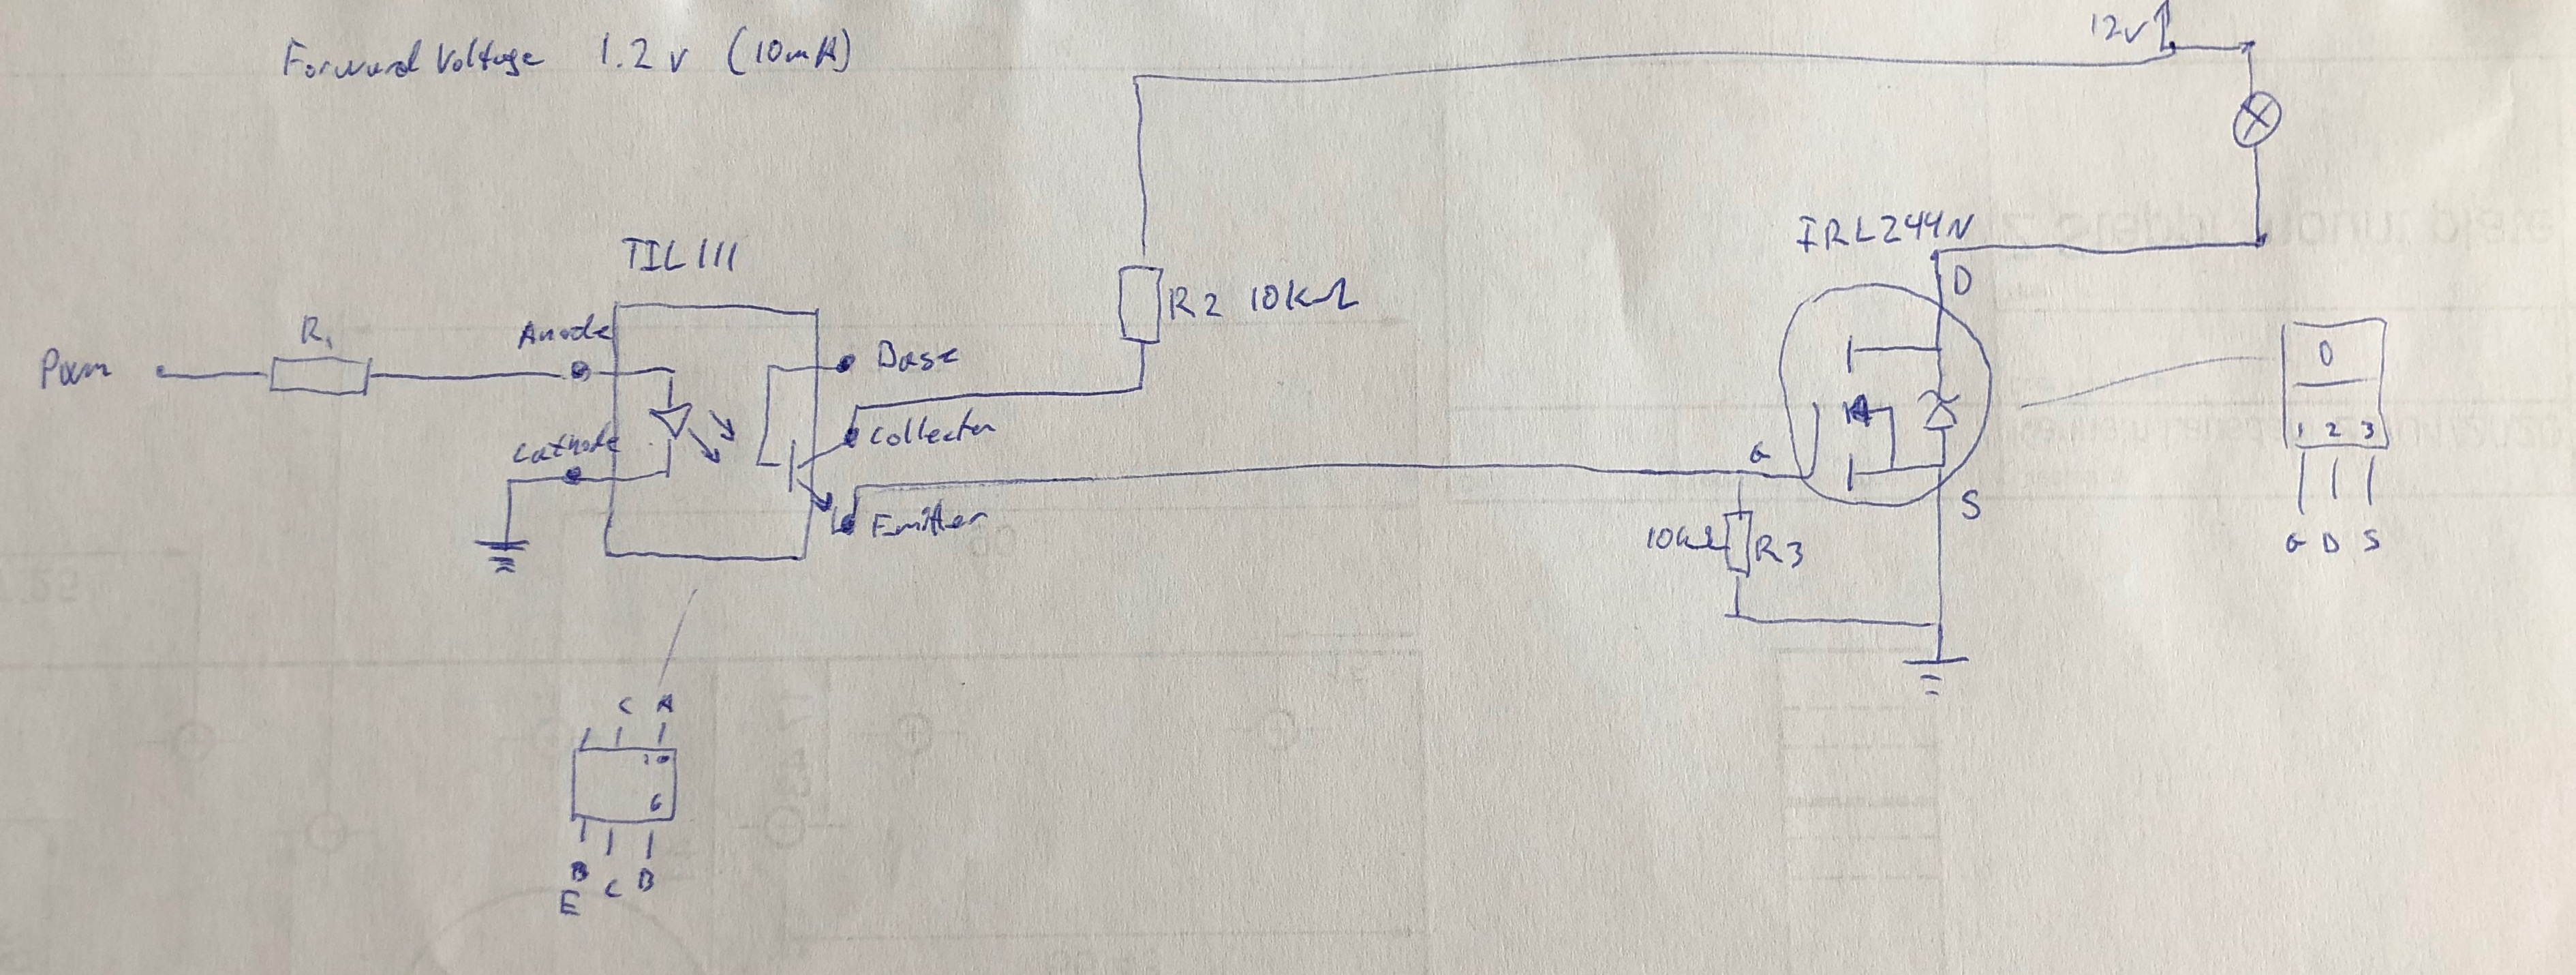
\includegraphics[scale=0.1]{IMG_1614.jpeg}

\caption{Overall design}
\label{fig:overallDesign}
\end{figure}


\subsection{Calculation of optocoupker resistor}

Spec for TIL111

\begin{enumerate}
	\item Forward Voltage 1.2v (10mA)
\end{enumerate}





\begin{equation}
 \begin{array}{l}
R = \frac{V}{I}\\
R_1 = \frac{3.3v -1.2v }{ 0.010A} = 210 \Omega 
\end{array}
\end{equation}

This means that the input resistor between the PI pin and the anote of the optocoupler must be at least 210 $\Omega$ so 220 $\Omega$ is a good candidate

\subsection{MOSFET}

Spec for IRLZ44N (N-channel mostfet:

\begin{enumerate}
	\item $R_{DS_{ON}}$ = 0.022$\Omega$ $V_{GS}=10v$ $I_D = 25A$
	\item $V_{GS}=16V$ max gate voltage
	\item 175 \degree{}C - max operation temp
	\item $V_{CS(th)} = 1v$
	\item $R_B{_JA}=62$ \degree{}C/W
\end{enumerate}

Heat disipation assuming a heated bed plate with this spec is powered:
\begin{enumerate}
	\item $R = 1.65\Omega$ for 12v
	\item $P = 87 w$
	\item $A=7.25A$
\end{enumerate}

Calculate watts for when powering the heated bed
\begin{equation}
 \begin{multlined}
P = R*I^2\\
 = 22mA*7.25^2 = 1156mW = 1.156W
\end{multlined}
\end{equation}

Calculate watts the MOSFET can handle withtout cooling
\begin{equation}
 \begin{multlined}
P_D = \frac{max(T_J)-T_A}{R_{øJA}}\\
= \frac{175\degree{}C-25\degree{}C}{62} = 2.4 W\\
\end{multlined}
\end{equation}

So to use it without a heat sink we need $1.156W < 2.4W$ which it is so no heat sink required.

Calculating resistors between the optocoupker and mosfet. Two resistors are required. One to pull down the gate when not powered here a $10K\Omega$ or similar is fine the smaller the faster it turns off. The other resistor is required to make a voltage devider to protect the gate input voltage of the MOSFET which has a max input voltage of $V_{GS} = 16v$. This means if we power it by 12v then nothing is needed but for other reasons a resistor should be added, bla bla.. So we chose to design it to also allow for 24v and get both handled by the same design.

A Voltage desiver is defined as
 \begin{equation}
 \begin{multlined}
V_{out} = \frac{V_s * R_2}{R_1+R_2}
\end{multlined}
\end{equation}

So lets find a resistor

 \begin{equation}
 \begin{multlined}
V_{out} = \frac{12v * 10K\Omega}{10K\Omega+10K\Omega} = 6v \\
 = \frac{24v * 10K\Omega}{10K\Omega+10K\Omega} = 12v 
\end{multlined}
\end{equation}
So we see that both of these gives a voltage less than $V_{gs}$ i.e. $12v < 16v$ so this resistor valye is fine. The value is also above $V_{CS(th)}$ so it is enough to turn it on


\subsection{A first version of the schematics}

\begin{figure}[!hpt]
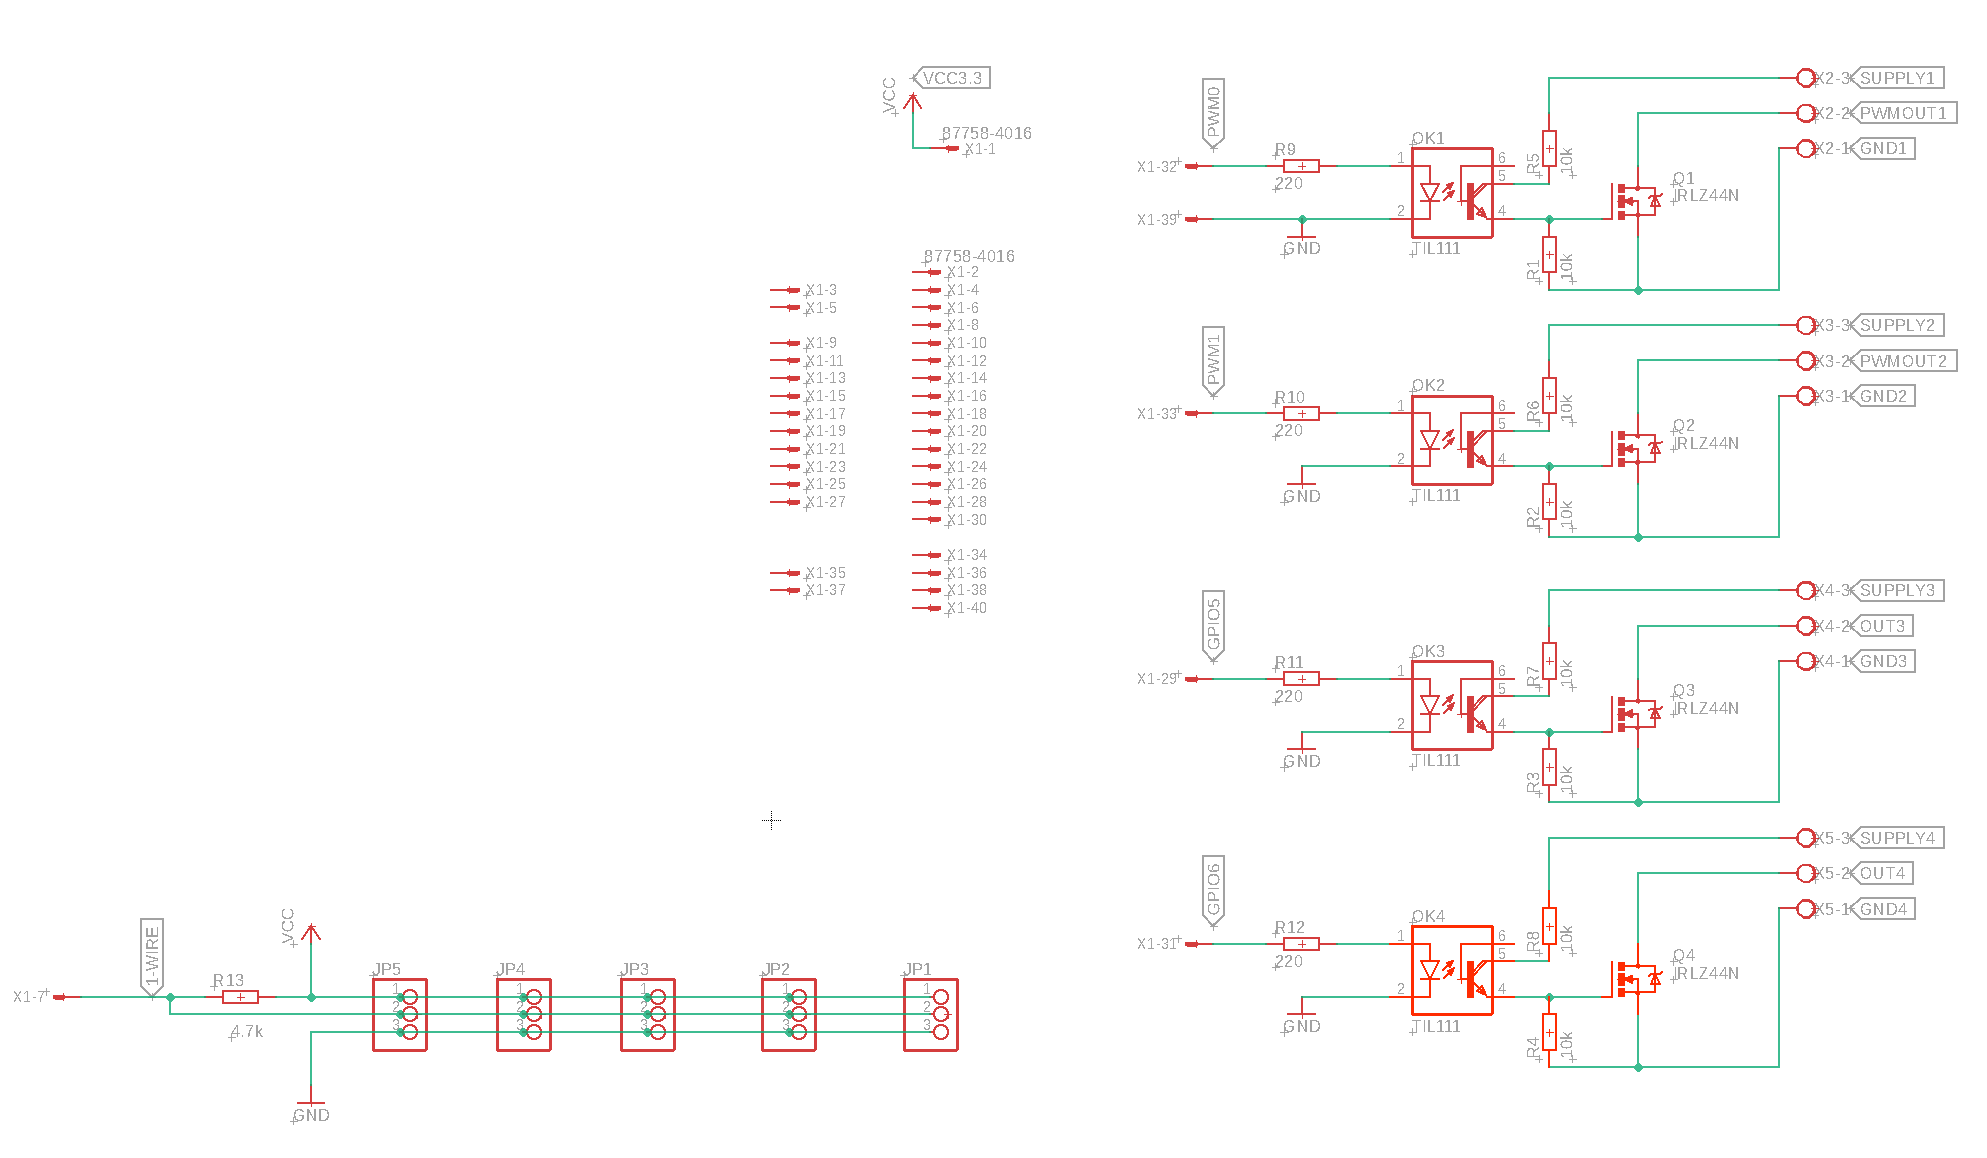
\includegraphics[scale=0.2]{schematics.png}

\caption{Schematics}
\label{fig:schematics}
\end{figure}

\end{document}
